\chapter{Sztuczna inteligencja - taktyki}\label{tacticts}
W grze symulacyjnej, będącej przedmiotem niniejszej pracy dyplomowej, terroryści oraz antyterroryści posiadają sztuczną inteligencję\footnote{charakterystyka modelu SI została przedstawiona w rozdziale \ref{aiModelInfo}}, która pozwala im na podejmowanie decyzji oraz poruszanie się. Interfejsem, z którego jednostki uczestniczące w symulacji czerpią wiedzę o świecie gry, jest obiekt Game. 

\section{Taktyka antyterrorystów}
Antyterroryści posiadają strategię, która nakazuje im posiadanie lidera przez cały czas trwania symulacji. Lider antyterrorystów jest jednostką, za którą w szyku poruszają się pozostali antyterroryści. Jeżeli lider zginie, to natychmiastowo wybierany jest nowy lider, a działania grupy są kontynuowane.

Antyterrorysta posiada skończony zbiór stanów (rysunek \ref{atTacticImage}), które odzwierciedlają podjęte przez niego decyzje i definiują jego działania. Po zainicjalizowaniu obiektu antyterrorysty przechodzi on do stanu \emph{follow entity}, który pozwala mu podążać za swoimi poprzednikami. Jest to domyślny stan, do którego antyterrorysta może wrócić ze stanów, do których przeszedł na podstawie zdarzenia. Jeżeli antyterrorysta jest liderem, to następuje natychmiastowe przejście do stanu \emph{follow path}, które definiuje konieczność poruszania się po wyznaczonej ścieżce do następnego punktu kluczowego. Wraz z dotarciem do danego punktu kluczowego, wyznaczana jest ściseżka do następnego punktu kluczowego. Jeżeli antyterrorysta lider dotarł do ostatniego punktu kluczowego, to zmienia on swój stan na \emph{follow extraction}, który nakazuje jednostce poruszanie się po ścieżce do punktu startowego / końcowego antyterrorystów. Po dotarciu do tego punktu antyterrorysta zatrzymuje się i przechodzi do stanu bezczynności - \emph{idle}.

\begin{figure}
\begin{center}
	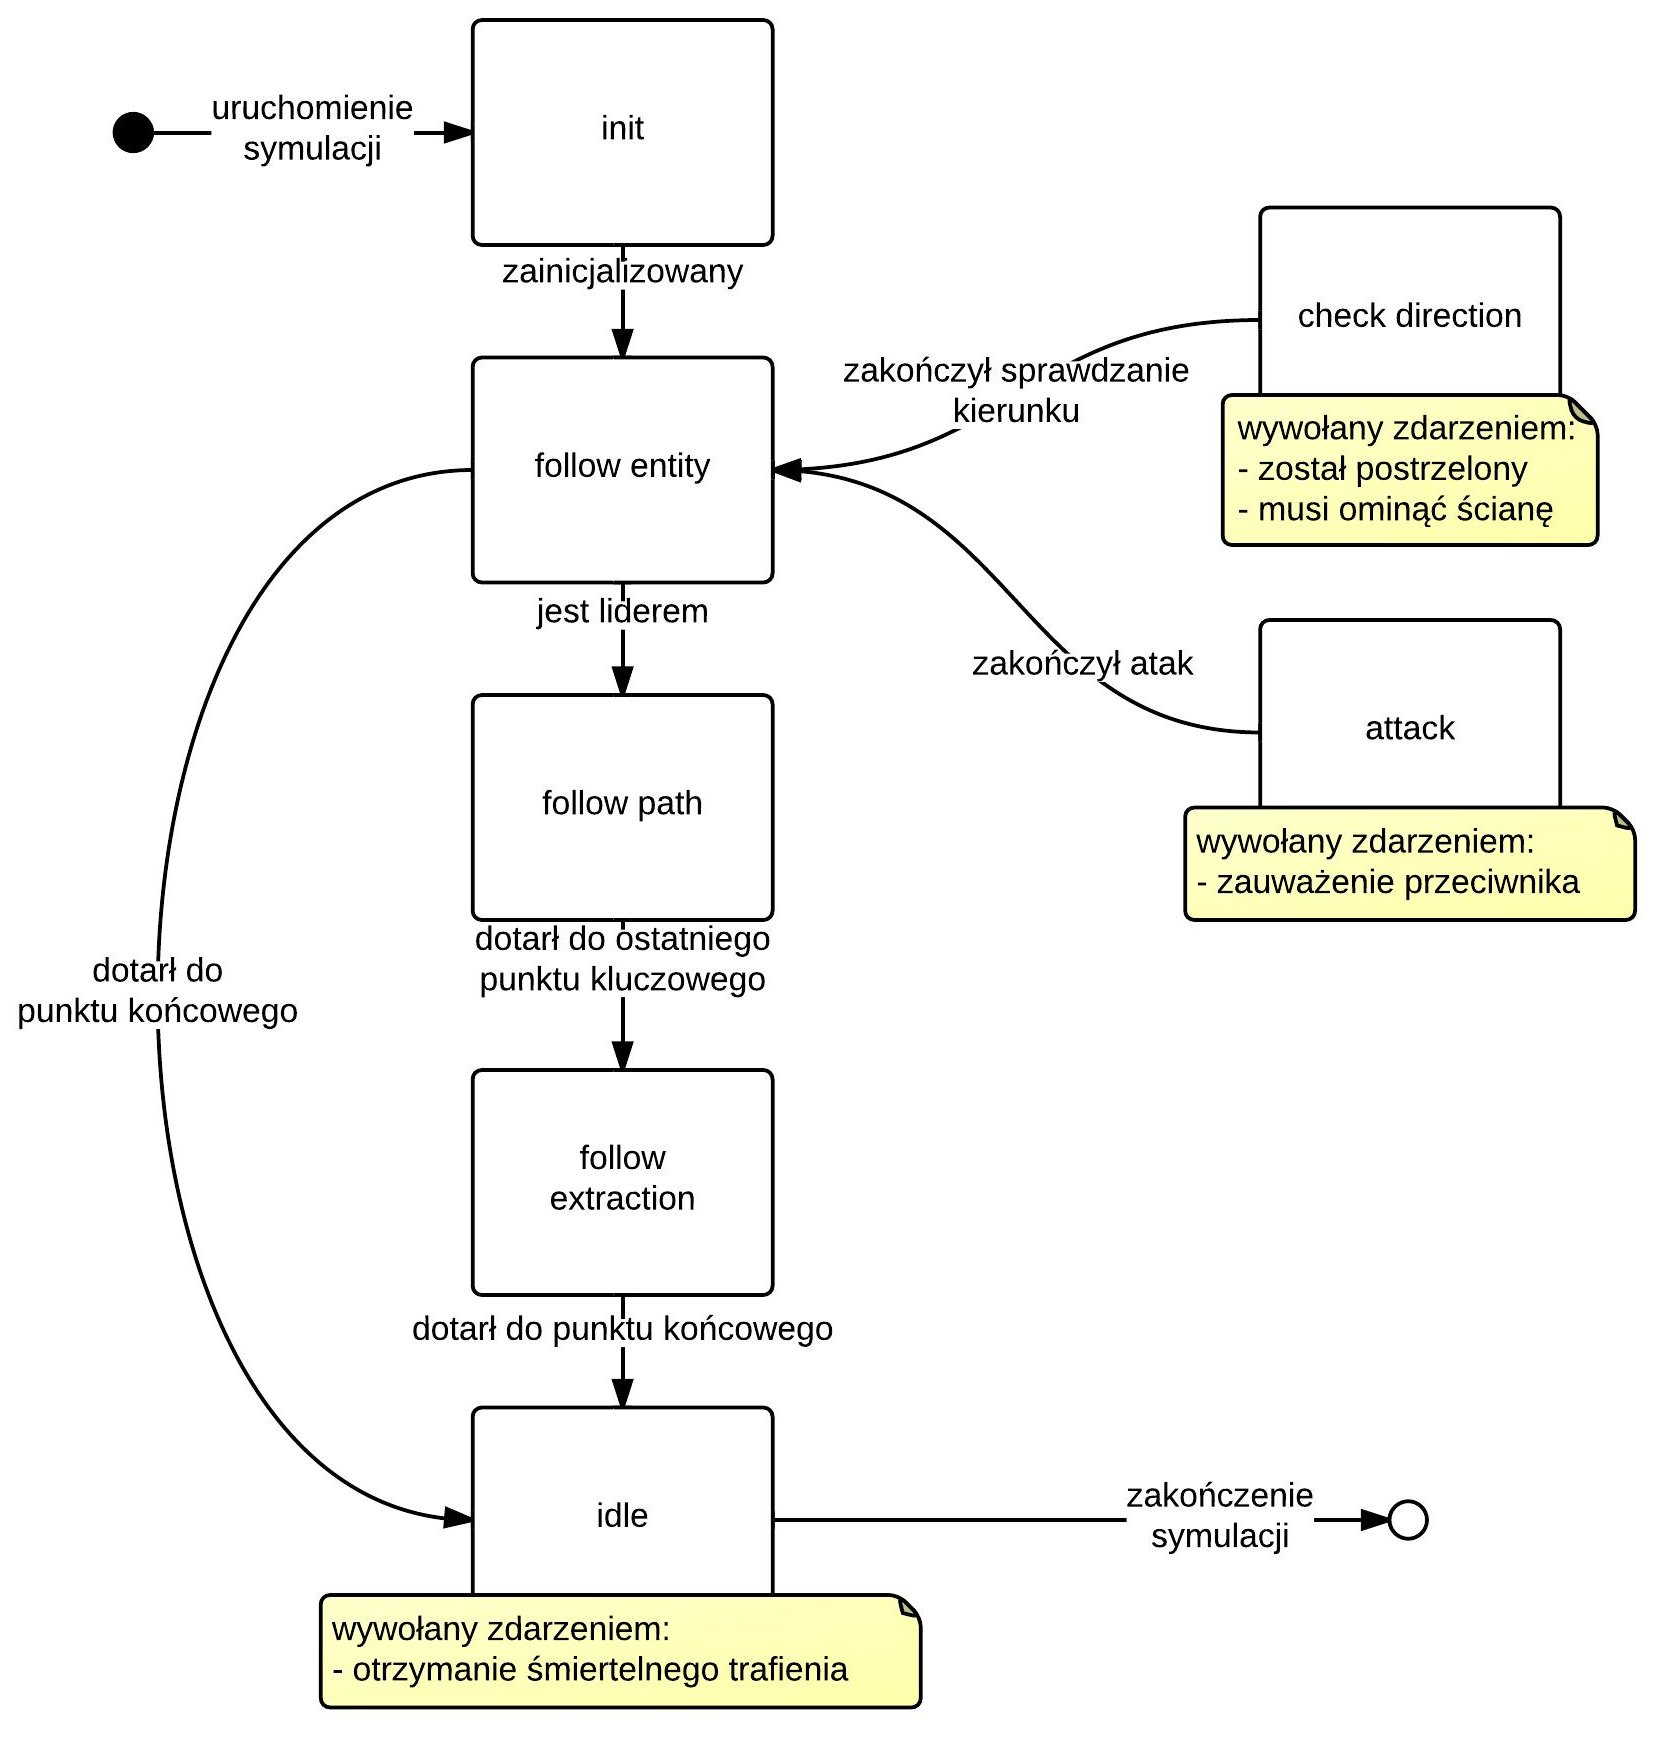
\includegraphics[width=160mm,height=105mm]{images/atTactic}
	\caption{Diagram przejść międzystanowych antyterrorysty\label{atTacticImage}}
\end{center}
\end{figure}

Każdy antyterrorysta może zmienić swój stan na podstawie zaistniałego zdarzenia. Postrzelenie antyterrorysty lub natrafienie przez niego na ścianę, wiąże się z~natychmiastowym wywołaniem stanu \emph{check location}. Stan ten definiuje poruszanie się jednostki do zadanego punktu, z wykorzystaniem wyliczonej ścieżki bezkolizyjnej. Antyterrorysta opuszcza ten stan po dotarciu do celu lub po upłynięciu limitu czasowego na wykonanie tej czynności. Zdarzenie polegające na zauważeniu przeciwnika, wywołuje stan \emph{attack}. Stan ten pozwala antyterroryście na oddawanie strzałów w kierunku zauważonego terrorysty, jeżeli na linii strzału nie znajduje się żaden antyterrorysta. Wyjście z tego stanu następuje po zabiciu terrorysty lub po straceniu celu z pola widzenia.

\section{Taktyka terrorystów}
Terroryści nie posiadają grupowej strategii działania, kierują się wyłącznie indywidualnie podejmowanymi decyzjami. Terrorysta posiada skończony zbiór stanów (rysunek \ref{terTacticImage}). Po zainicjalizowaniu obiektu terrorysty przechodzi on do stanu \emph{wander}, który pozwala mu na wędrowanie po świecie gry. Podczas wędrowania terrorysta może podjąć decyzję o~wykonaniu postoju, co wiąże się z przejściem do stanu \emph{stand}. Stan ten zatrzymuje jednostkę oraz odlicza czas pozostały do końca postoju, a po jego upłynięciu zmienia stan terrorysty ponownie na \emph{wander}.

\begin{figure}
\begin{center}
	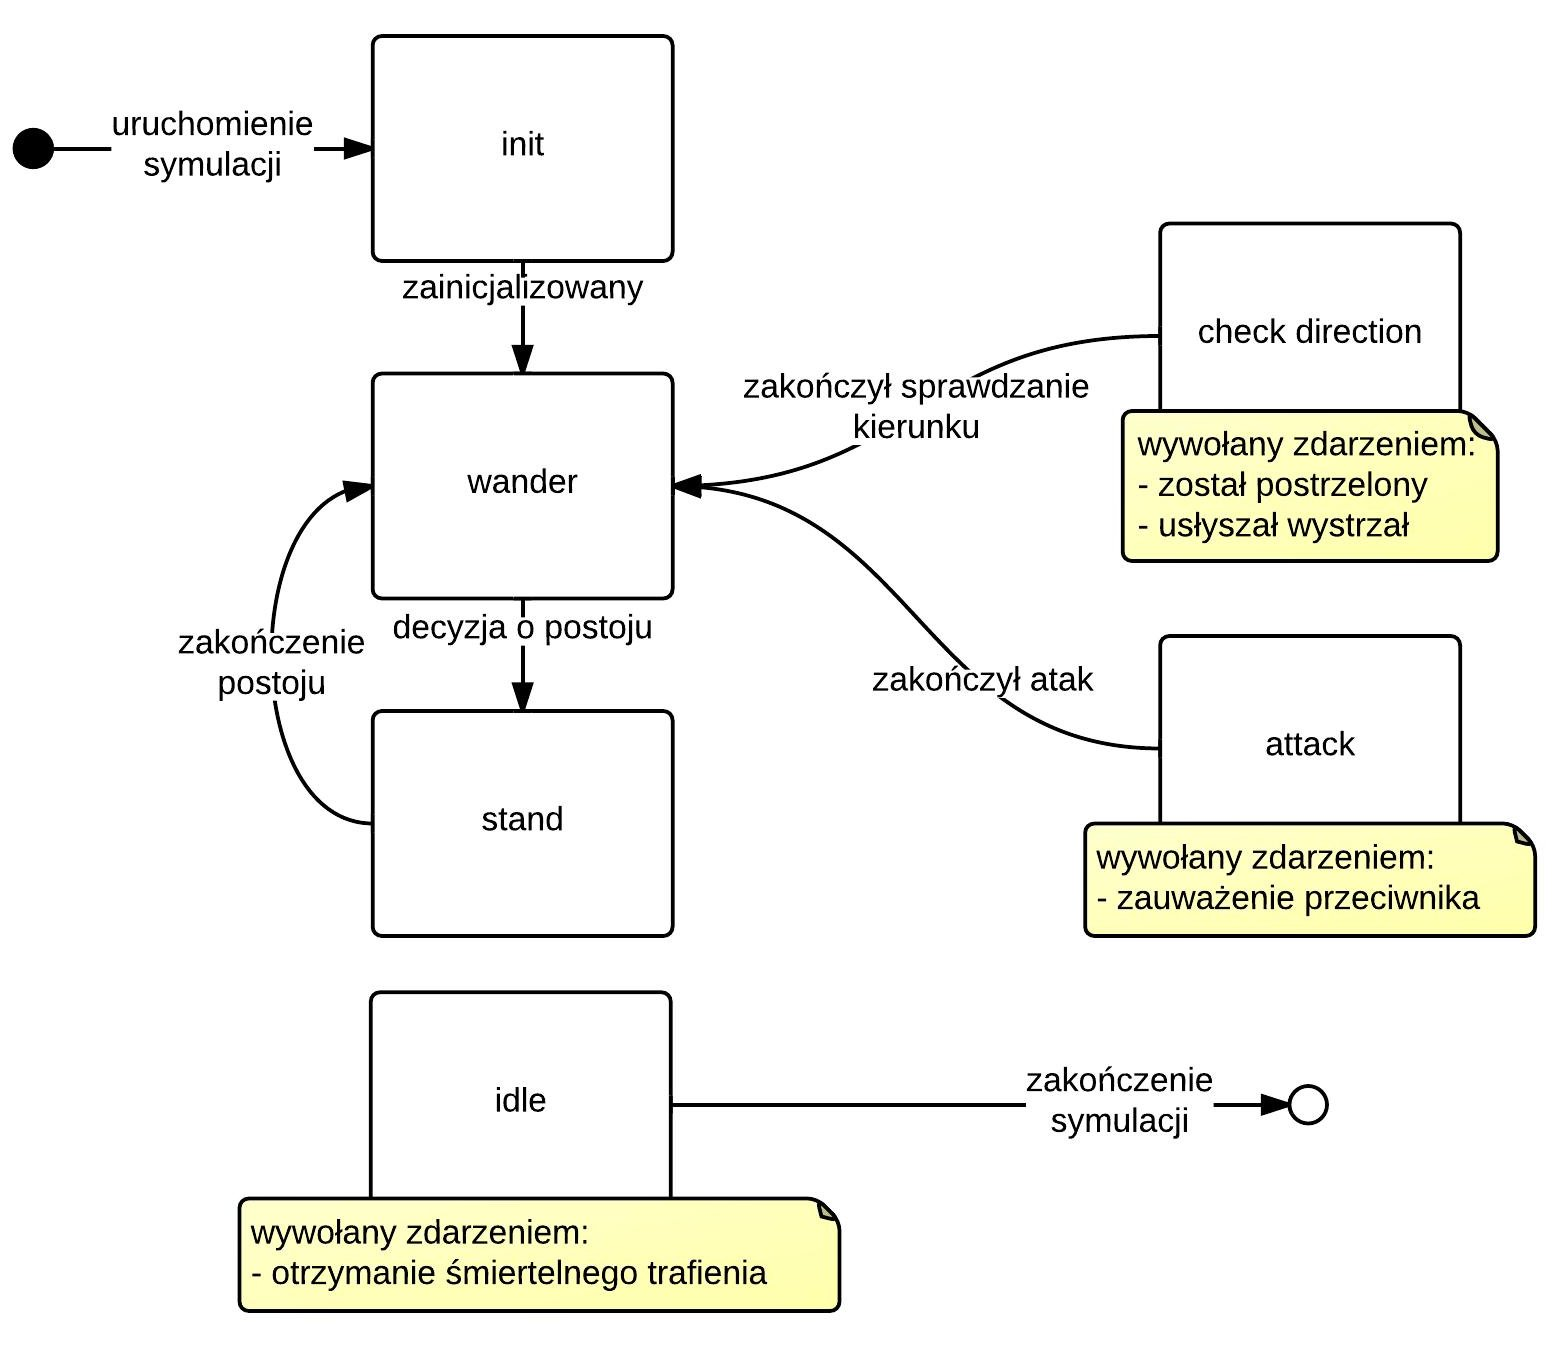
\includegraphics[width=160mm,height=84mm]{images/terTactic}
	\caption{Diagram przejść międzystanowych terrorysty\label{terTacticImage}}
\end{center}
\end{figure}

Każdy terrorysta także może zmienić swój stan na podstawie zaistniałego zdarzenia. Postrzelenie terrorysty lub usłyszenie przez niego odgłosu wystrzału skutkuje wywołaniem stanu \emph{check location}, który definiuje identyczne zachowanie i warunek wyjścia ze stanu, jak w przypadku antyterrorysty. Podobnie jest ze zdarzeniem polegającym na zauważeniu przeciwnika. Wywołuje ono stan \emph{attack}, który nakazuje terroryście strzelać do wrogiej jednostki. Warunek wyjścia z tego stanu jest taki sam, jak u antyterrorysty.

Zdarzeniem wspólnym dla antyterrorystów oraz dla terrorystów jest otrzymanie śmiertelnego trafienia. W tym przypadku natychmiastowo zmieniany jest stan jednostki na bezczynność - \emph{idle}. Jednostka pozostająca w stanie bezczynności nie reaguje na zdarzenia, co skutkuje brakiem możliwości zmiany swego stanu.


\section{Opis algorytmów}
W tym rozdziale zostaną przedstawione wybrane algorytmy, jakie są wykorzystywane w grze symulacyjnej, będącej przedmiotem tej pracy dyplomowej. Słowny opis jest uzupełniony pseudokodami lub implementacją w języku Javascript.

\subsection{Myślenie i poruszanie się jednostek}
Antyterroryści i terroryści w grze symulacyjnej posiadają zaimplementowaną metodę \emph{think} pozwalającą na realizację działań zapisanych w konkretnych stanach (listing \ref{thinkAt} oraz \ref{thinkTer}). Prócz wywołania metod odpowiadającym konkretnym stanom, wywoływane są także metody \emph{watchForEnemy} oraz \emph{checkForCollision}. Ta pierwsza pozwala jednostce na obserwowanie otoczenia w poszukiwaniu przeciwników, natomiast druga na bezpieczne omijanie ścian. Metody odpowiadające za realizację poszczególnych stanów podejmują najczęściej decyzję, gdzie leży następny cel jednostki.

\begin{table}
\begin{center}
\begin{lstlisting}
    think: function(){
        this.watchForEnemy();
        switch(this.currentState) {
            case 'idle': break;
            case 'init': this.setup(); break;
            case 'follow entity': this.followEntity(); break;
            case 'follow path': this.followPath(); break;
            case 'follow extraction': this.followExtraction(); break;
            case 'check location': this.checkLocation(); break;
            case 'attack': this.attack(); break;
            default: this.changeToDefaultState(); break;
        }
        if (this.avoiding) this.wanderOrientation = this.getRotation();
        this.avoiding = this.checkForCollision();
    }
 \end{lstlisting}
\caption {Metoda think w klasie Game.Antiterrorist}
\label{thinkAt}
\end{center}
\end{table}

\begin{table}
\begin{center}
\begin{lstlisting}
    think: function(){
        this.watchForEnemy();
        switch(this.currentState) {
            case 'idle': break;
            case 'init': this.setup(); break;
            case 'stand': this.stand(); break;
            case 'wander': this.wander(); break;
            case 'check location': this.checkLocation(); break;
            case 'attack': this.attack(); break;
            default: this.changeToDefaultState(); break;
        }
        if (this.avoiding) this.wanderOrientation = this.getRotation();
        this.avoiding = this.checkForCollision();
    }
 \end{lstlisting}
\caption {Metoda think w klasie Game.Terrorist}
\label{thinkTer}
\end{center}
\end{table}

Gdy cel jest już zdefiniowany, to wykonywane są algorytmy niższego poziomu, odpowiedzialne za obliczenie wektora prędkości oraz prędkości, z jaką ma poruszać się jednostka. Takimi algorytmami są \emph{seek} (ruch w kierunku celu) oraz \emph{flee} (ruch w przeciwnym kierunku do celu). Metoda think jest wywoływana wewnątrz metody \emph{update} (listing \ref{update}), która służy do zmiany pozycji obiektu na scenie. Po wykonaniu metody \emph{think} zmieniana jest aktualna pozycja obiektu o wyliczony wektor prędkości, natomiast orientacja obiektu jest uaktualniana, by była zgodna z wektorem prędkości. Aktualizacja pozycji i orientacji nie następuje, gdy gra jest w trybie pauzy lub dany obiekt ruchomy już nie żyje.

\begin{table}
\begin{center}
\begin{lstlisting}
    update: function(frame) {
        if (!Game.paused && this.isAlive) {
            this.think();
            if (this.hasVelocity()) {
                this._updateCollisionRay();
                var pos = this.getVecPosition().add(this.getVecVelocity().multiply(frame.timeDiff * this.speed));
                this.setPosition(pos.e(1),pos.e(2));
                var rot = Math.atan2(-this.getVecVelocity().e(1), this.getVecVelocity().e(2));
                this.setRotation(rot);
            }
        }
   }
 \end{lstlisting}
\caption {Metoda update w klasie Game.Entity}
\label{update}
\end{center}
\end{table}

Metoda update jest wywoływana w anonimowej funkcji, przypisanej do zdarzenia zmiany klatki animacji\footnote{definicja obsługi tego zdarzenia znajduje się w metodzie Game.init()}. Obsługa tego zdarzenia stanowi główną pętlę aplikacji. Co klatkę następuje iteracja po wszystkich warstwach przypisanych do sceny (listing \ref{onFrame}). Dla każdej warstwy interujemy po wszystkich obiektach, jakie zostały dodane do danej warstwy. Jeżeli obiekt posiada zdefiniowaną metodę update (co oznacza, że jego klasa dziedziczy z Game.Entity), to jest ona wykonywana. Po przetworzeniu wszystkich obiektów w danej warstwie, wykonywana jest metoda draw, która renderuje ponownie warstwę na scenie.

\begin{table}
\begin{center}
\begin{lstlisting}
    this.stage.onFrame(function(frame) {
          for(var layerIndex in self.stage.getChildren()) {
              var layer = self.stage.getChildren()[layerIndex];
              for (var objectIndex in layer.getChildren()) {
                  var object = layer.getChildren()[objectIndex];
                  if(object.update) object.update(frame);
              }
              layer.draw();
          }
    });
 \end{lstlisting}
\caption {Rysowanie klatek animacji}
\label{onFrame}
\end{center}
\end{table}

\subsection{Wyznaczanie ścieżki - A*}\label{graph}
Wyznaczanie ścieżek bezkolizyjnych (uwzględniających położenie ścian na mapie) jest realizowane poprzez algorytm A*, który na bazie grafu jest w stanie odnaleźć drogę między dwoma zadanymi węzłami. W grze symulacyjnej graf zawiera węzły, które mogą mieć przypisany jeden z dwóch stanów: otwarty lub zamknięty. Wyliczona ścieżka nigdy nie prowadzi przez węzły zamknięte.

Algorytm został opisany przez Petera Harta, Nilsa Nilssona oraz Bertrama Raphaela w 1968 roku i początkowo nosił nazwę \emph{A}. Jednakże ze względu na zastosowanie heurystyki, polegającej na przeszukiwaniu grafu z pierwszeństwem analizy węzłów obiecujących (tj. tych, które znajdują się bliżej węzła docelowego), nadano algorytmowi nazwę \emph{A*}.

W grze symulacyjnej wykorzystywana jest javascript'owa implementacja algorytmu A*, przygotowana przez Briana Grinsteada w formie biblioteki javascript-astar\cite{astarPage}. Inicjalizacja grafu oraz przykład wyszukiwania ścieżki zostały przedstawione w listingu \ref{astarCode}. W definicji grafu \emph{1} oznacza węzeł otwarty, a \emph{0} węzeł zamknięty. Podczas definiowania przez użytkownika konfiguracji symulacji, w miejscu gdzie jest postawiona ściana węzły grafu zmieniają swój typ na zamknięty. Wynikiem wyszukiwania jest uporządkowana lista węzłów, jakie jednostka musi odwiedzić w drodze do celu. Algorytm wyznaczania scieżki jest zaimplementowany w metodzie \emph{calculatePath} klasy Game.Entity.

\begin{table}
\begin{center}
\begin{lstlisting}
	var graph = new Graph([
		[1,1,1,1,1,1,1,1,1,1],
		[1,1,1,1,0,0,1,1,1,1],
		[1,1,1,1,0,0,1,1,1,1],
		[1,1,1,1,0,0,1,1,1,1],
		[1,1,1,1,1,1,1,1,1,1],
	]);
	var start = graph.nodes[0][0];
	var end = graph.nodes[9][4];
	var result = astar.search(graph.nodes, start, end);
 \end{lstlisting}
\caption {Inicjalizacja grafu 10x5 oraz wyszukiwanie ścieżki między węzłami}
\label{astarCode}
\end{center}
\end{table}

\subsection{Zauważanie przeciwnika}\label{detectionSubsection}

\begin{figure}
\begin{center}
	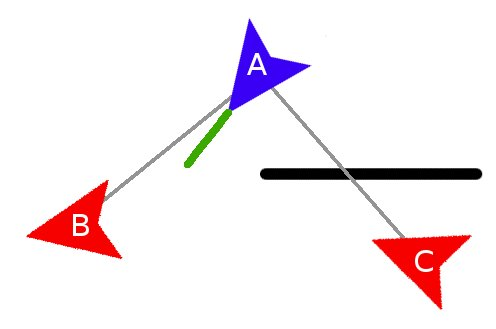
\includegraphics[width=80mm,height=53mm]{images/detection}
	\caption[Zauważanie przeciwnika]{Zauważanie przeciwnika: Najbliższym przeciwnikiem jednostki A jest jednostka B. Jednostka C nie jest analizowana, ponieważ znajduje się za ścianą. Zielona linia to linia sprawdzająca ew. kolizje dla jednostki A\label{detectionImage}}
\end{center}
\end{figure}

Algorytm zauważania przeciwnika jest zaimplementowany w metodzie \emph{closestSeenOpponent} klasy Game.Entity. Zwraca on referencję do najbliższego przeciwnika, będącego w zasięgu wzroku. Algorytm iteruje po liście przeciwników, dokonując szeregu sprawdzeń tylko dla tych jednostek, które jeszcze żyją. Tzw. \emph{dłuższy dystans} obliczany jest między pozycją obserwującej jednostki a pozycją potencjalnego przeciwnika. \emph{Krótszy dystans} obliczany jest między końcem linii sprawdzającej ew. kolizje dla jednostki obserwującej a pozycją potencjalnego przeciwnika (rysunek \ref{detectionImage}). Jeżeli \emph{krótszy dystans} jest rzeczywiście mniejszy od \emph{dłuższego dystansu}, to oznacza to, że przeciwnik jest przed jednostką obserwującą\footnote{jednostki będące za plecami jednostki obserwującej są ignorowane}. Jeżeli dystans pomiędzy jednostkami jest większy od zasięgu wzroku lub jest większy niż zapamiętany dystans do aktualnego celu, to taki przeciwnik jest ignorowany. Jeżeli jednak odległości są mniejsze, a przeciwnik nie znajduje się za jakąkolwiek ścianą, to oznaczamy go za cel i zapamiętujemy nowy, aktualny dystans do celu. Pseudokod algorytmu jest zapisany w~listingu \ref{detectionCode}.

\begin{table}
\begin{center}
\begin{lstlisting}
	cel = null
	dystans_do_celu = ja.zasieg_wzroku
	DLA KAZDEGO przeciwnik z lista_przeciwnikow WYKONUJ
		JEZELI przeciwnik.nie_zyje TO wykonaj_nastepna_iteracje
		dluzszy_dystans = oblicz_dystans (ja.pozycja, przeciwnik.pozycja)
		krotszy_dystans = oblicz_dystans (ja.koniec_promienia_kolizji, przeciwnik.pozycja)
		JEZELI krotszy_dystans < dluzszy_dystans ORAZ krotszy_dystans < dystans_do_celu TO
			JEZELI lista_scian_na_drodze (ja.pozycja, przeciwnik.pozycja) JEST PUSTA TO
				cel = przeciwnik
				dystans_do_celu = krotszy_dystans		
	ZWROC cel	
\end{lstlisting}
\caption {Pseudokod algorytmu zauważania przeciwnika}
\label{detectionCode}
\end{center}
\end{table}

\subsection{Podążanie jednostek w linii}

\begin{figure}
\begin{center}
	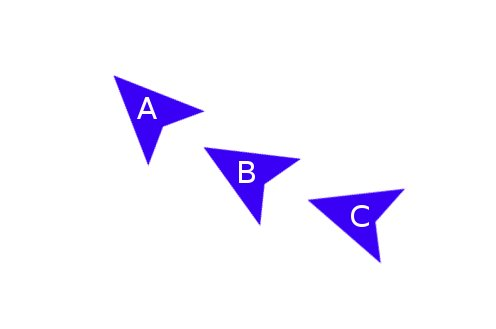
\includegraphics[width=80mm,height=53mm]{images/followEntity}
	\caption[Podążanie jednostek w linii]{Podążanie jednostek w linii: Jednostka A jest liderem. Z jednostką A, w określonym odstępie porusza się jednostka B, natomiast za jednostką B porusza się jednostka C\label{followEntityImage}}
\end{center}
\end{figure}

Antyterroryści w grze symulacyjnej poruszają się w szyku liniowym (rysunek \ref{followEntityImage}). Taka kolumna zaatakowana bezpośrednio od przodu lub od tyłu ma najmniejszą siłę ogniową. Linia zaatakowana od boku posiada bardzo dużą siłę ogniową, bowiem antyterroryści nie zasłaniają sobie na wzajem celu. Algorytm podążania w linii jest zaimplementowany w metodzie \emph{followEntity} klasy Game.Antiterrorist. Próbuje on dla danej jednostki znaleźć przyjazną jednostkę, która ją poprzedza i nie zginęła. Jeżeli taka jednostka nie zostanie znaleziona, to oznacza to, że dana jednostka jest liderem i należy zmienić jej stan na \emph{follow path}. W przeciwnym wypadku dana jednostka wylicza i podąża do współrzędnych celu, które są iloczynem odległości podążania oraz różnicy aktualnej pozycji znalezionego sprzymierzeńca i jego wektora prędkości. Pseudokod algorytmu jest zapisany w~listingu \ref{followEntityCode}.

\begin{table}
\begin{center}
\begin{lstlisting}
	indeks = ja.indeks_w_grupie
	POWTARZAJ
		indeks = indeks - 1
		sprzymierzeniec = sprzymierzency[indeks]
	DOPOKI (ISTNIEJE(sprzymierzeniec) ORAZ sprzymierzeniec.nie_zyje)
	JEZELI (NIE_ISTNIEJE(sprzymierzeniec)) TO
		ja.jestLiderem = PRAWDA
		ja.zmien_stan('follow path')
	WPP
		ja.jednostka_cel = sprzymierzeniec

	ja.pozycja_celu = (sprzymierzeniec.wektor_pozycji - sprzymierzeniec.wektor_predkosci) * ja.odleglosc_podazania
	ja.seek()
\end{lstlisting}
\caption {Pseudokod algorytmu podążania za jednostką}
\label{followEntityCode}
\end{center}
\end{table}

\subsection{Atakowanie jednostki}
Atak na wrogą jednostkę jest poprzedzany obserwacją, która przeprowadzana jest niezależnie od stanu, w jakim znajduje się aktualnie jednostka. Z tego algorytmu korzystają zarówno antyterroryści, jak i terroryści. Jest on zaimplementowany w~metodzie \emph{watchForEnemy} klasy Game.Entity. Na początku metoda korzysta z~algorytmu zauważania przeciwnika (rozdział \ref{detectionSubsection}). Jeżeli dana jednostka nie widzi w~danym momencie potencjalnego przeciwnika, a obecnie znajduje się w stanie \emph{attack}, to następuje przejście do stanu domyślnego tej jednostki. Jednak gdy przeciwnik został znaleziony, ale nie był wcześniej obserwowany, to dana jednostka rozpoczyna jego obserwację ustawiając czas do ataku na zdefiniowany w parametrach czas reakcji. Gdy jednak znaleziony przeciwnik jest już obserwowany i upłynie czas do ataku, to dana jednostka przechodzi do stanu \emph{attack}, jeżeli tylko nie ma przed sobą żadnych sprzymierzeńców stojących na linii ognia. Pseudokod algorytmu jest zapisany w listingu \ref{watchForEnemyCode}.

\begin{table}
\begin{center}
\begin{lstlisting}
	najblizszy_przeciwnik = znajdz_najblizszego_przeciwnika();
	JEZELI (NIE_ISTNIEJE(najblizszy_przeciwnik)) TO
		JEZELI (ja.aktualny_stan == 'attack')
			ja.pozycja_celu = null
			ja.zmien_stan_na_domyslny()
	WPP
		JEZELI (najblizszy_przeciwnik != ja.obserwowany_przeciwnik) TO
			ja.obserwowany_przeciwnik = najblizszy_przeciwnik
			ja.czas_do_ataku = ja.czas_reakcji
		WPP
			ja.czas_do_ataku = ja.czas_do_ataku - 1
			JEZELI (ja.czas_do_ataku < 0) TO
				JEZELI lista_sprzymierzencow_na_drodze (ja.pozycja, najblizszy_przeciwnik.pozycja) JEST PUSTA TO
					ja.jednostka_cel = najblizszy_przeciwnik
					ja.zmien_stan('attack')									
\end{lstlisting}
\caption {Pseudokod algorytmu obserwowania wroga}
\label{watchForEnemyCode}
\end{center}
\end{table}

Realizacja ataku polega na wystrzeliwaniu pocisku co określony interwał czasowy. Jeżeli upływa czas do kolejnego strzału, to tworzona jest nowa instancja pocisku, którego pozycja i orientacja są zgodne z odpowiednikami u strzelca. Obiekt pocisku wykonuje metodę \emph{move}, która sprawdza, czy pocisk nie trafił w ścianę lub jednostkę. W tym drugim przypadku zadawane są obrażenia zgodnie z energią, jaką posiadał pocisk w momencie trafienia. Pseudokod algorytmu ataku jest zapisany w listingu \ref{attackCode}.

\begin{table}
\begin{center}
\begin{lstlisting}
	ja.uaktualnij_pozycje_cel()
	ja.seek()				
	JEZELI (ja.czas_do_strzalu < 0) TO
		ja.czas_do_strzalu = ja.czas_miedzy_strzalami
		strzelec = ja
		UTWROZ('pocisk', strzelec)
	ja.czas_do_strzalu = ja.czas_do_strzalu - 1;
\end{lstlisting}
\caption {Pseudokod algorytmu atakowania wroga}
\label{attackCode}
\end{center}
\end{table}

\subsection{Sprawdzanie lokacji}

W szczególnych przypadkach jednostki mogą przejść do stanu \emph{check location}, którego definicja nakazuje przejście jednostki do zadanego miejsca na mapie. Przed przejściem do tego stanu jest ustawiany cel i obliczana bezkolizyjna ścieżka do niego (listing \ref{checkLocationSet}). Dla antyterrorystów przejście do stanu \emph{check location} jest wywoływane w następujących sytuacjach:
\begin{itemize}
	\item antyterrorysta nie będący liderem natrafi na ścianę, która odgradza go od antyterrorysty poprzednika; wyznaczanym celem jest pozycja poprzednika na mapie
	\item antyterrorysta otrzyma trafienie; wyznaczanym celem jest pozycja strzelca na mapie
\end{itemize}

Terroryści również korzystają z implementacji stanu \emph{check location}. W ich przypadku stan ten jest wywoływany gdy:
\begin{itemize}
	\item terrorysta usłyszy odgłos wystrzału lub trafienia; wyznaczanym celem jest pozycja pocisku w momencie wystrzału lub trafienia
	\item antyterrorysta otrzyma trafienie; wyznaczanym celem jest pozycja strzelca na mapie
\end{itemize}

Jednostki posiadają ograniczony czas na przejście do zadanej lokacji (listing \ref{checkLocationDo}). Antyterroryści posiadają bardzo niską wartość maksymalnego czasu na sprawdzenie lokacji, gdyż priorytetem dla nich jest wykonanie planu poruszając się w grupie, gdzie posiadają większą siłę ognia. Warunkiem wyścia ze stanu jest upłynięcie czasu na sprawdzenie lokacji lub dotarcie do niej. Jednostka opuszczająca stan \emph{check location} przechodzi do własnego domyślnego stanu.

\begin{table}
\begin{center}
\begin{lstlisting}
	ja.czas_na_sprawdzenie_lokacji = ja.maksymalny_czas_na_sprawdzenie_lokacji
	ja.wytycz_sciezke_do(cel)
	ja.zmien_stan('check location')
\end{lstlisting}
\caption {Pseudokod algorytmu sprawdzania lokacji (metoda setCheckLocation)}\label{checkLocationSet}
\label{attackCode}
\end{center}
\end{table}


\begin{table}
\begin{center}
\begin{lstlisting}
	wezel = sciezka[ja.indeks_wezla]
	JEZELI (ja.czas_na_sprawdzenie_lokacji < 0 LUB NIE_ISTNIEJE(wezel)) TO
		ja.zmien_stan_na_domyslny()	
	WPP
		ja.pozycja_celu = wspolrzedne_wezla(wezel)
		JEZELI (ja.dotarl_do_celu) TO
			ja.indeks_wezla = ja.indeks_wezla + 1
		ja.czas_na_sprawdzenie_lokacji = ja.czas_na_sprawdzenie_lokacji - 1
		ja.seek()	
\end{lstlisting}
\caption {Pseudokod algorytmu sprawdzania lokacji (metoda checkLocation)}\label{checkLocationDo}
\label{attackCode}
\end{center}
\end{table}
